\chapter{Experiments}

% Short introduction such as: this chapter describes how the tests should be
% conducted, explain thorougly the scheduler script, gathered data etc.
\section{Proposed workflow and methodology}

[PLACEHOLDER]
% Here explain, what should be done in order to conduct measurements and make sure 
% No one taints them! Enumerate the ideas from the research paper / seminar i.e.
% Reservartion of node, request and fail of setting the fans to full speed etc.

% HERE TALK ABOUT WHICH BENCHMARK ARE BEING RUN AND THE CONFIGS
% Remind about the chosen benchmarks and configs 

\section{Working environment $-$ servers details}

[PLACEHOLDER]
% Describe more thoroughly the nodes: CPUs, GPUs, RAM, PSUs, PM connection etc

\section{Main tests}

\subsection{Overview on the scheduler script}

Things to explain:
1. Dictionaries with configs, that work for both choosing the right config and
provides path to save measurements
2. Section that run CPUs benchmarks, GPUs benchmarks, perf, nvml, yoko
3. Functions that check if the benchmarks are still running
4. Function that cleans-up every process after tests


\subsection{Main automation function \- scheduler()}

% NOTE TO SELF: Make sure this chart belongs to this section

\begin{figure}[hbtp]
    \centering
    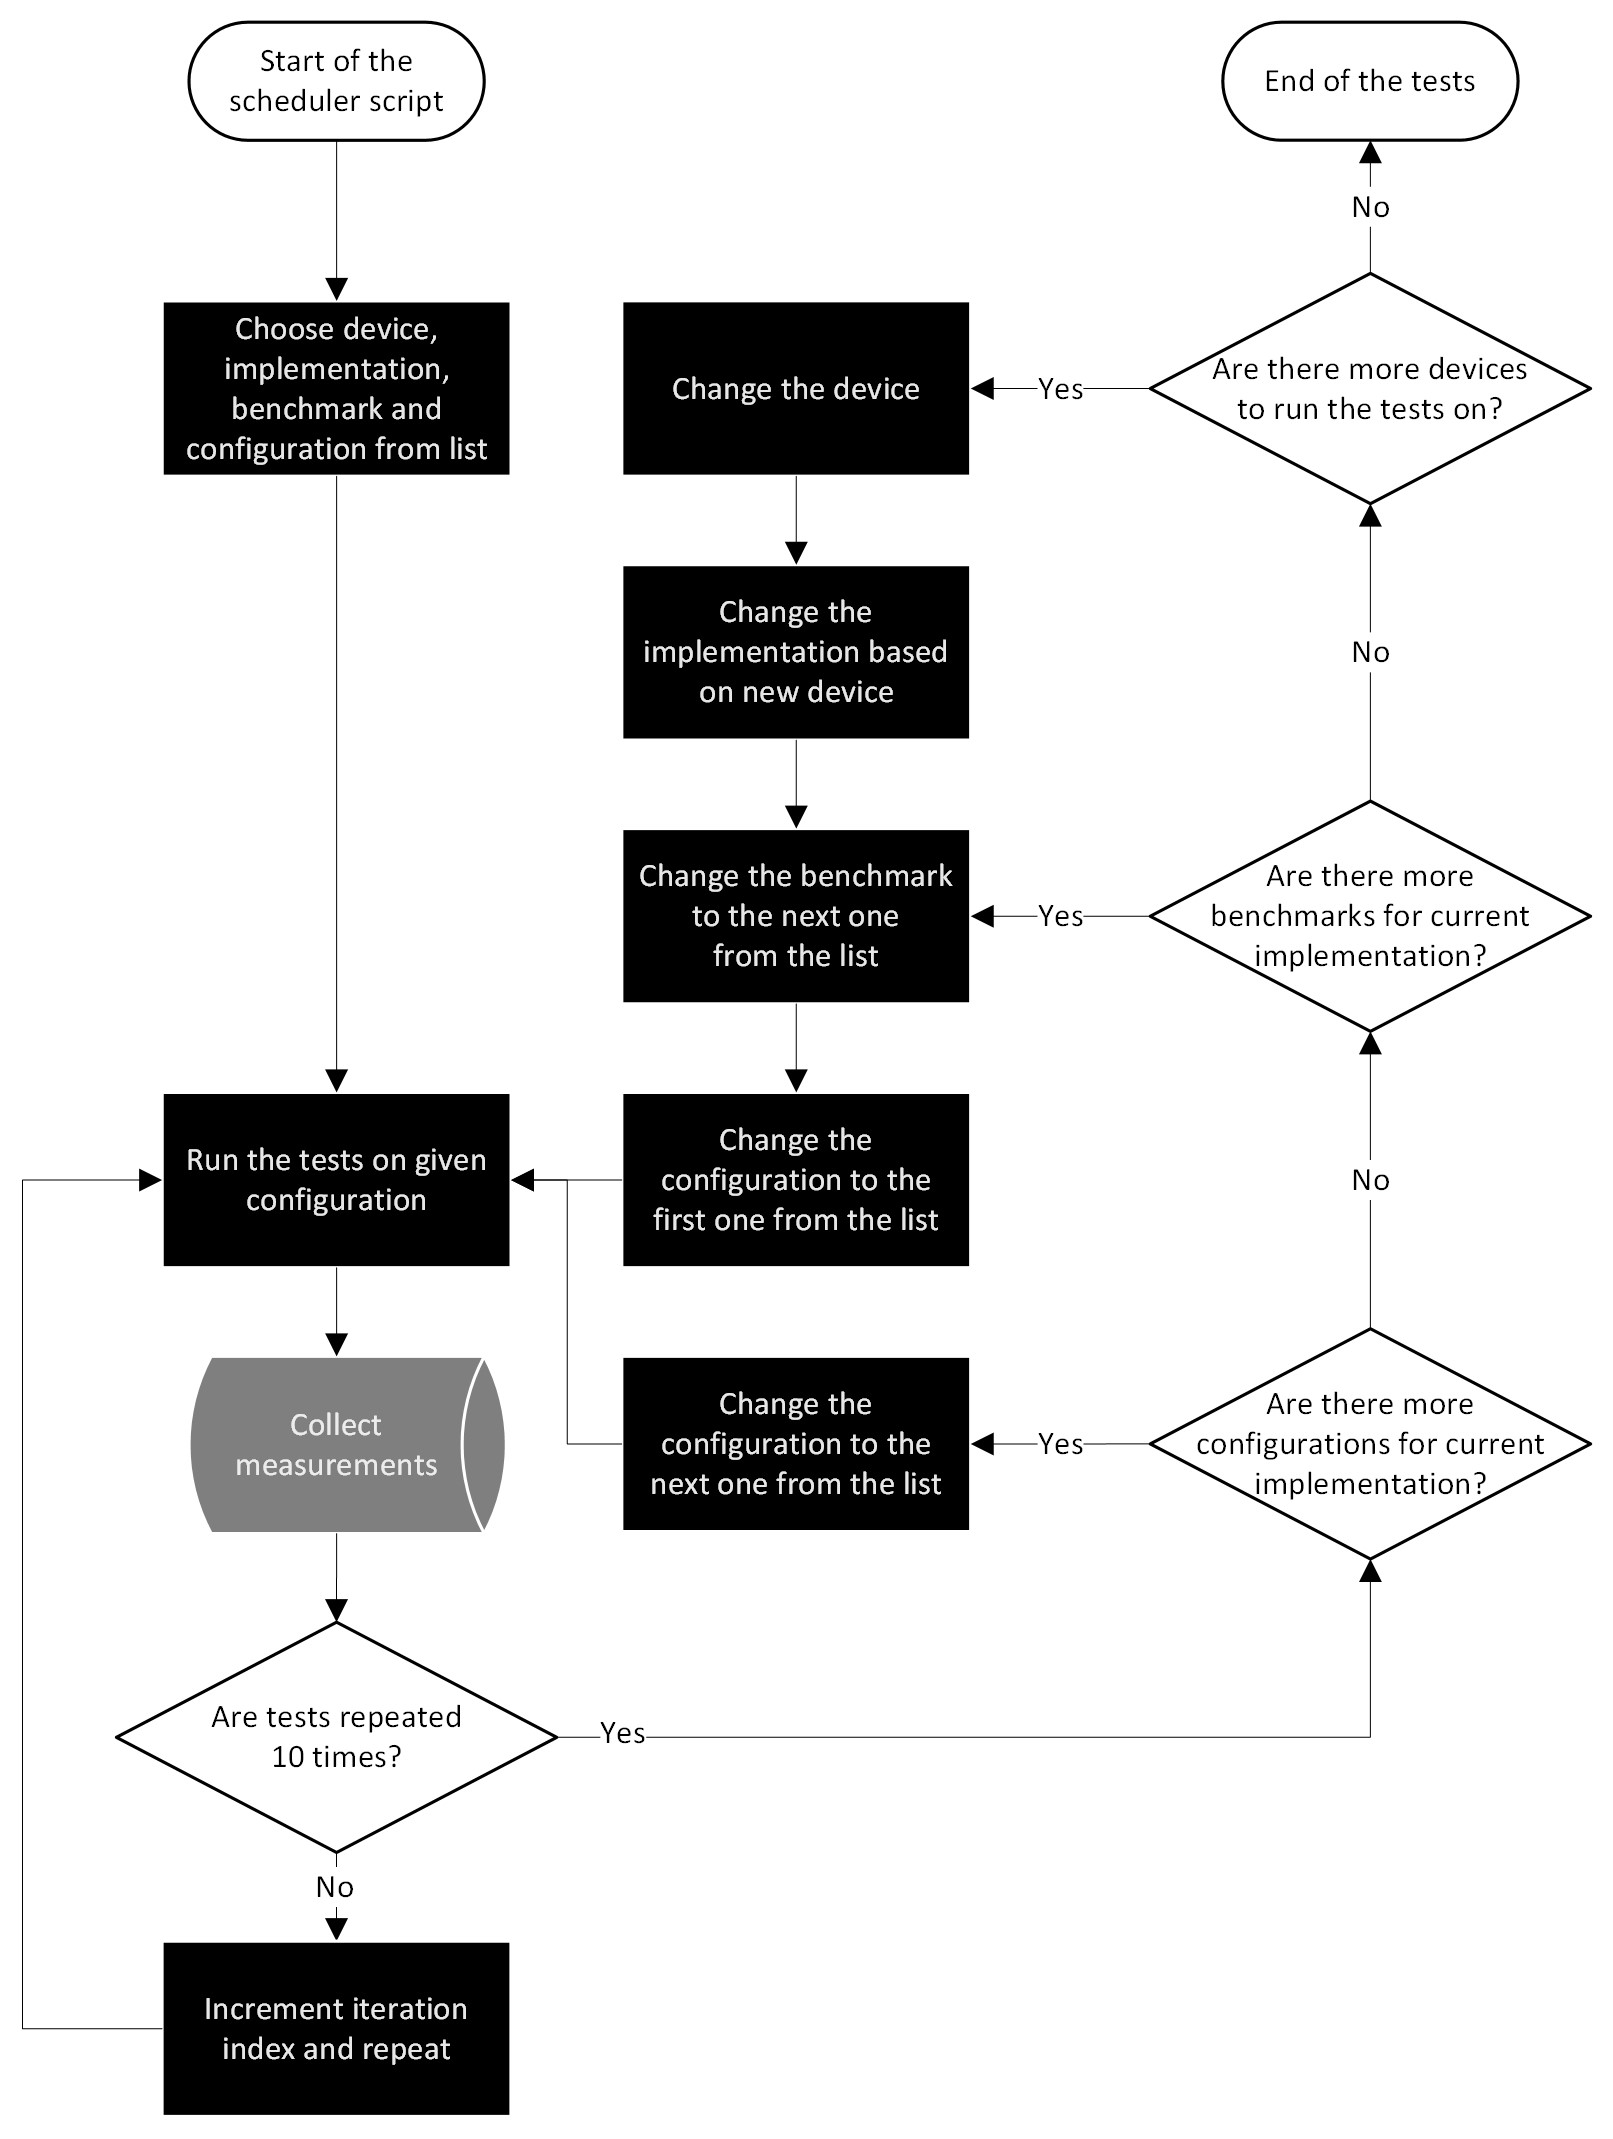
\includegraphics{general_flowchart}
    \caption{General Flowchart}~\label{fig:general_flowchart}
\end{figure}


\subsection{Threads pinning and kernels execution \- cpu\_benchmark()}

\begin{figure}[hbtp]
    \centering
    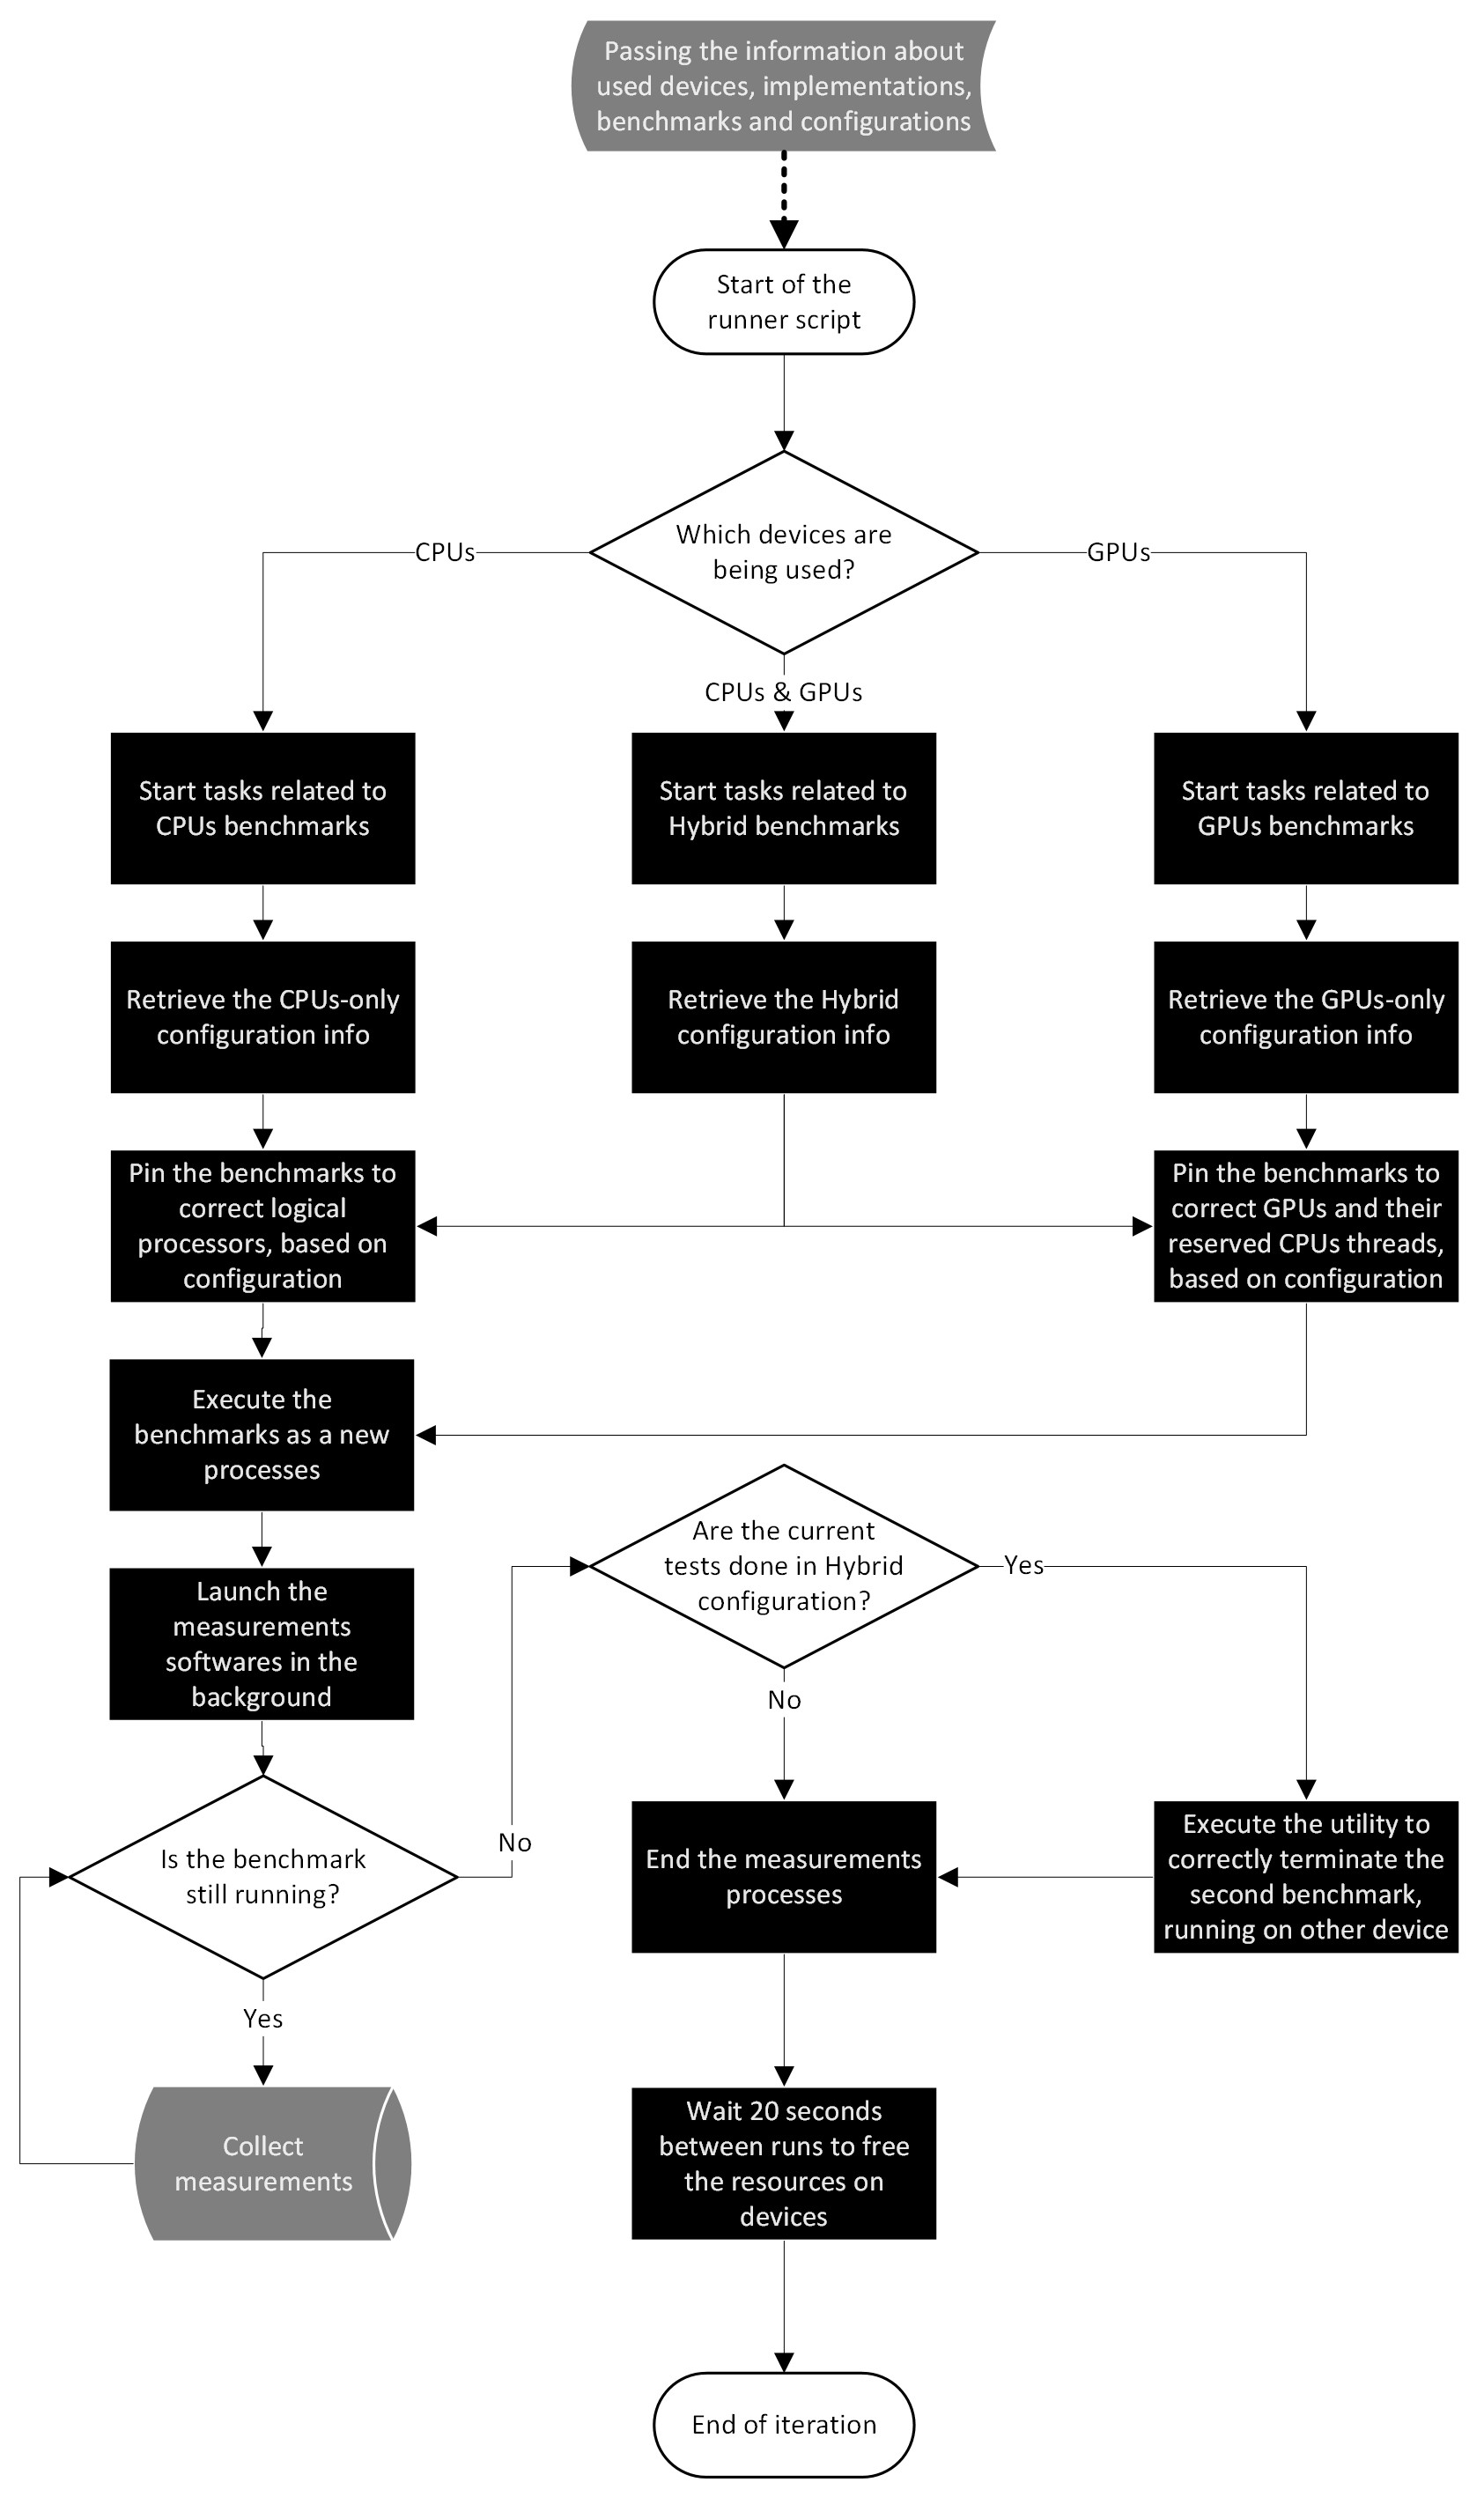
\includegraphics{processes_flowchart.jpeg}
    \caption{Processes Flowchart}~\label{fig:processes_flowchart.jpeg}
\end{figure}

% ===================

\subsection{GPUs and threads management \- gpu\_benchmark()}

\subsection{Measurements with Yokotool software \- yoko()}

\subsection{Measurements with Linux Perf software \- perf()}

\subsection{Measurements with NVML handling function \- nvml()}

\subsection{Cleanup of measurements daemons}

\subsection{Termination of benchmarks in Hybrid configuration}

% psutil

[PLACEHOLDER]
% Put the charts and plots of received measurements

\section{Analysis of the results and discussion}

[PLACEHOLDER]
% Put the analysis of the received data, according to Dr. Czarnul